% Continual-phase spectra + singular-vector alignment, all four CL sequences
% (rebuttal promise to 9k3u, W2). Numbers from scripts/make_cl_alignment_figure.py;
% per-stage numbers in tables/tab_cl_spectra_alignment.tex / cl_spectra_alignment.md.
% Pick ONE of path A or path B.

% =====================================================================
% PATH A (recommended): one compact figure replaces Fig. 16 (Setup 4 only,
% one full page) and covers all four sequences in ~0.55 page; add the table.
% =====================================================================
\begin{figure}[t]
  \centering
  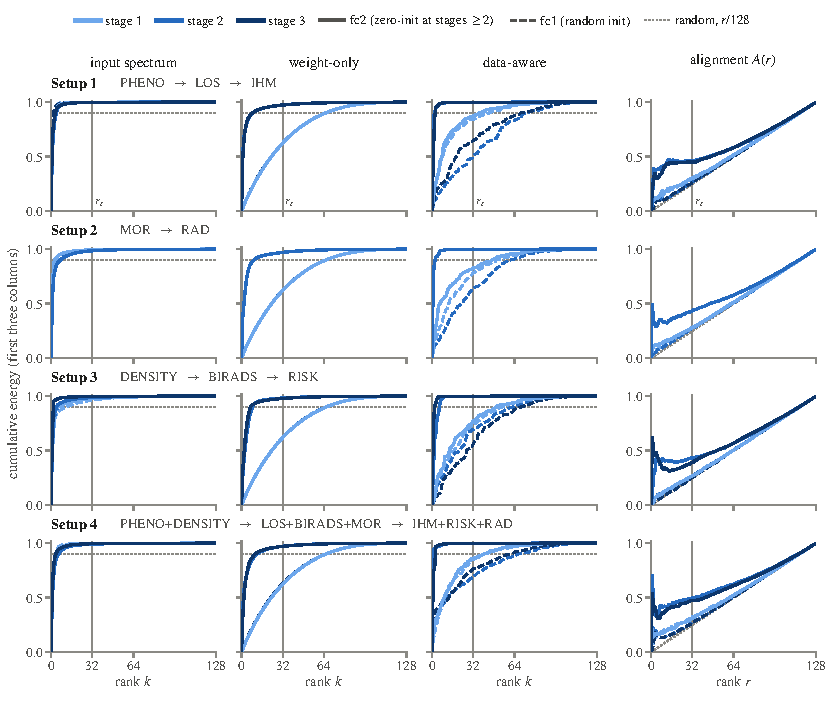
\includegraphics[width=\linewidth]{figs/fig_cl_spectra_alignment.pdf}
  \caption{Continual-stage spectra and singular-vector alignment for the four CL sequences
  (rows; FLAME-CL, seed 42). For the active component of each stage under that stage's routed
  inputs: input spectrum of $C_i$, weight-only spectrum $\sigma_{i,k}^2$, data-aware energy
  $E_{i,k}=\sigma_{i,k}^2 v_{i,k}^\top C_i v_{i,k}$ (cumulative, as in Fig.~3), and the alignment
  $A(r)=\lVert V_r^\top Q_r\rVert_F^2/r$ between the top-$r$ right singular vectors of the
  component and the top-$r$ eigenvectors of $C_i$ (dotted: random subspaces, $r/128$). Each line
  is the median over the 5 experts; solid fc2, dashed fc1; colour = stage. At stages $\geq 2$ fc2
  is zero-initialised (the setting of Proposition~2), fc1 keeps its default random
  initialisation, and at stage~1 both start from random initialisation. Vertical line: $r_t=32$.
  $C_i$ is estimated on the first $\leq 512$ validation samples of each task of the stage.
  Per-stage numbers in Tab.~\ref{tab:cl-spectra-alignment}.}
  \label{fig:cl-spectra-alignment}
\end{figure}
% + \begin{table}[t]
\centering
\scriptsize
\setlength{\tabcolsep}{3.2pt}
\caption{Continual-phase spectra and singular-vector alignment of the active component of each stage (FLAME-CL, seed 42), median over the 5 experts, reported as fc2\,/\,fc1. $r_{90}$: rank at 90\% cumulative energy (ambient 128). Kept: data-aware energy inside the top-32 singular directions, i.e.\ what survives the $r_t{=}32$ truncation. $A(r)=\lVert V_r^\top Q_r\rVert_F^2/r$ between the top-$r$ right singular vectors of the component and the top-$r$ eigenvectors of its routed-input second moment; random subspaces give $r/128$ (0.125 at $r{=}16$, 0.25 at $r{=}32$). fc2 is zero-initialised at stages $\geq$2; fc1, and both sublayers at stage 1, start from random init.}
\label{tab:cl-spectra-alignment}
\begin{tabular}{@{}llccccc@{}}
\toprule
 & & \multicolumn{3}{c}{$r_{90}$ (fc2\,/\,fc1)} & Kept at $r_t{=}32$ & $A(16)$ \\
\cmidrule(lr){3-5}
Setup & Stage & input & weight-only & data-aware & data-aware & (random 0.125) \\
\midrule
1 & 1: PHENO & 4\,/\,4 & 65\,/\,66 & 37\,/\,45 & 0.87\,/\,0.84 & 0.21\,/\,0.20 \\
 & 2: LOS & 5\,/\,3 & 9\,/\,65 & 2\,/\,74 & 1.00\,/\,0.51 & 0.46\,/\,0.14 \\
 & 3: IHM & 4\,/\,2 & 9\,/\,65 & 3\,/\,69 & 1.00\,/\,0.65 & 0.44\,/\,0.15 \\
\addlinespace[2pt]
2 & 1: MOR & 3\,/\,7 & 66\,/\,66 & 47\,/\,50 & 0.83\,/\,0.78 & 0.17\,/\,0.17 \\
 & 2: RAD & 8\,/\,7 & 10\,/\,66 & 3\,/\,62 & 1.00\,/\,0.64 & 0.36\,/\,0.15 \\
\addlinespace[2pt]
3 & 1: DENSITY & 6\,/\,12 & 66\,/\,65 & 50\,/\,55 & 0.77\,/\,0.74 & 0.16\,/\,0.15 \\
 & 2: BIRADS & 5\,/\,6 & 9\,/\,66 & 6\,/\,62 & 1.00\,/\,0.69 & 0.41\,/\,0.16 \\
 & 3: RISK & 2\,/\,2 & 7\,/\,66 & 2\,/\,69 & 1.00\,/\,0.56 & 0.32\,/\,0.12 \\
\addlinespace[2pt]
4 & 1: PHENO+DENSITY & 4\,/\,4 & 66\,/\,66 & 41\,/\,41 & 0.86\,/\,0.85 & 0.21\,/\,0.23 \\
 & 2: LOS+BIRADS+MOR & 7\,/\,5 & 12\,/\,66 & 1\,/\,68 & 1.00\,/\,0.69 & 0.44\,/\,0.16 \\
 & 3: IHM+RISK+RAD & 4\,/\,5 & 11\,/\,65 & 3\,/\,61 & 1.00\,/\,0.76 & 0.41\,/\,0.16 \\
\bottomrule
\end{tabular}
\end{table}


% Replacement text for App. D.4.3 (first paragraph; the "cannot be read off the weight
% spectrum alone ... Tab. 4" ending can stay as is):
\paragraph{D.4.3 Continual-Stage Spectra and Alignment.}
Fig.~\ref{fig:cl-spectra-alignment} repeats the three-lens diagnostic in the continual phase for
all four sequences, for the active component of each stage under that stage's routed inputs, and
adds the singular-vector alignment of Proposition~2. The routed-input spectrum reaches 90\% of
its energy by rank~4 (median over all 110 stage sublayers, at most 22) at every stage of every
sequence, so Proposition~1's premise holds throughout each stream. The weight-only and data-aware
spectra split by initialization. At stages $\geq 2$ the output sublayer fc2 of each new component
is zero-initialized, the setting of Proposition~2: its data-aware energy reaches 90\% by rank~3
(range 1--8), the rank-32 truncation keeps $\geq 99.8\%$ of it, and its right singular vectors
align with the eigenvectors of $C_i$ well above chance ($A(16)=0.41$, range 0.22--0.51, against
0.125 for random subspaces). The input sublayer fc1 keeps its default random initialization, as
do both sublayers at stage~1, which trains from scratch. fc1 stays near chance alignment
($A(16)=0.16$) and accumulates data-aware energy gradually (90\% at rank~66), so the truncation
keeps a median 65\% of its data-aware energy; the stage-1 sublayers sit in between (90\% at
rank~46, 82\% kept, $A(16)=0.18$). Setup~4 gives the same picture on all four seeds
(Tab.~\ref{tab:cl-spectra-alignment}).
Functional rank therefore cannot be read off the weight spectrum alone, and the decisive test is
behavioral: [keep the existing ending about Proposition 5 and Tab. 4].

% =====================================================================
% PATH B: keep Fig. 16 exactly as it is and add the same-format pages for
% Setups 1-3, plus a one-row alignment figure. ~3 extra pages.
% The PNG titles and these subcaptions use 0-based stages, as Fig. 16 does.
% =====================================================================
\begin{figure}[p]
  \centering
  \begin{subfigure}{\linewidth}\centering
    \includegraphics[width=\linewidth]{figs/fig16_setup1_stage0.png}\caption{Stage 0: \{PHENO\}.}
  \end{subfigure}
  \begin{subfigure}{\linewidth}\centering
    \includegraphics[width=\linewidth]{figs/fig16_setup1_stage1.png}\caption{Stage 1: \{LOS\}.}
  \end{subfigure}
  \begin{subfigure}{\linewidth}\centering
    \includegraphics[width=\linewidth]{figs/fig16_setup1_stage2.png}\caption{Stage 2: \{IHM\}.}
  \end{subfigure}
  \caption{Continual-stage spectra for Setup 1; panels as in Fig.~16.}
\end{figure}
\begin{figure}[p]
  \centering
  \begin{subfigure}{\linewidth}\centering
    \includegraphics[width=\linewidth]{figs/fig16_setup2_stage0.png}\caption{Stage 0: \{MOR\}.}
  \end{subfigure}
  \begin{subfigure}{\linewidth}\centering
    \includegraphics[width=\linewidth]{figs/fig16_setup2_stage1.png}\caption{Stage 1: \{RAD\}.}
  \end{subfigure}
  \caption{Continual-stage spectra for Setup 2; panels as in Fig.~16. eICU samples contribute
  five routed tokens each, so $C_i$ is estimated from 64 test batches instead of 10.}
\end{figure}
\begin{figure}[p]
  \centering
  \begin{subfigure}{\linewidth}\centering
    \includegraphics[width=\linewidth]{figs/fig16_setup3_stage0.png}\caption{Stage 0: \{DENSITY\}.}
  \end{subfigure}
  \begin{subfigure}{\linewidth}\centering
    \includegraphics[width=\linewidth]{figs/fig16_setup3_stage1.png}\caption{Stage 1: \{BIRADS\}.}
  \end{subfigure}
  \begin{subfigure}{\linewidth}\centering
    \includegraphics[width=\linewidth]{figs/fig16_setup3_stage2.png}\caption{Stage 2: \{RISK\}.}
  \end{subfigure}
  \caption{Continual-stage spectra for Setup 3; panels as in Fig.~16.}
\end{figure}
\begin{figure}[t]
  \centering
  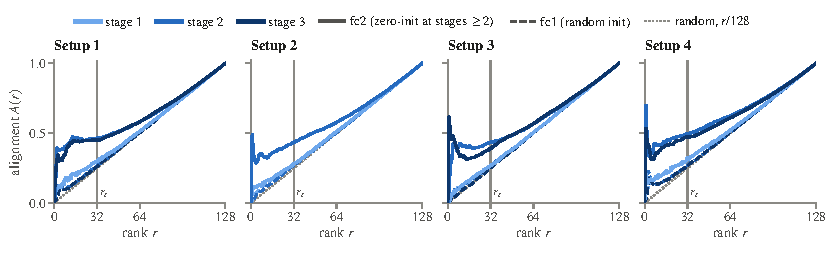
\includegraphics[width=\linewidth]{figs/fig_cl_alignment.pdf}
  \caption{Singular-vector alignment $A(r)=\lVert V_r^\top Q_r\rVert_F^2/r$ between the top-$r$
  right singular vectors of each stage's active component and the top-$r$ eigenvectors of its
  routed-input second moment $C_i$, for the four CL sequences (median over the 5 experts; solid
  fc2, dashed fc1; colour = stage; dotted: random subspaces, $r/128$). At stages $\geq 2$ the
  zero-initialised fc2 aligns well above chance ($A(16)=0.41$ vs.\ 0.125), as Proposition~2
  predicts; the randomly initialised fc1, and both sublayers at stage 1, stay near chance.
  Stages numbered from 1 here (stage 1 = stage 0 of Fig.~16).}
  \label{fig:cl-alignment}
\end{figure}
% + \begin{table}[t]
\centering
\scriptsize
\setlength{\tabcolsep}{3.2pt}
\caption{Continual-phase spectra and singular-vector alignment of the active component of each stage (FLAME-CL, seed 42), median over the 5 experts, reported as fc2\,/\,fc1. $r_{90}$: rank at 90\% cumulative energy (ambient 128). Kept: data-aware energy inside the top-32 singular directions, i.e.\ what survives the $r_t{=}32$ truncation. $A(r)=\lVert V_r^\top Q_r\rVert_F^2/r$ between the top-$r$ right singular vectors of the component and the top-$r$ eigenvectors of its routed-input second moment; random subspaces give $r/128$ (0.125 at $r{=}16$, 0.25 at $r{=}32$). fc2 is zero-initialised at stages $\geq$2; fc1, and both sublayers at stage 1, start from random init.}
\label{tab:cl-spectra-alignment}
\begin{tabular}{@{}llccccc@{}}
\toprule
 & & \multicolumn{3}{c}{$r_{90}$ (fc2\,/\,fc1)} & Kept at $r_t{=}32$ & $A(16)$ \\
\cmidrule(lr){3-5}
Setup & Stage & input & weight-only & data-aware & data-aware & (random 0.125) \\
\midrule
1 & 1: PHENO & 4\,/\,4 & 65\,/\,66 & 37\,/\,45 & 0.87\,/\,0.84 & 0.21\,/\,0.20 \\
 & 2: LOS & 5\,/\,3 & 9\,/\,65 & 2\,/\,74 & 1.00\,/\,0.51 & 0.46\,/\,0.14 \\
 & 3: IHM & 4\,/\,2 & 9\,/\,65 & 3\,/\,69 & 1.00\,/\,0.65 & 0.44\,/\,0.15 \\
\addlinespace[2pt]
2 & 1: MOR & 3\,/\,7 & 66\,/\,66 & 47\,/\,50 & 0.83\,/\,0.78 & 0.17\,/\,0.17 \\
 & 2: RAD & 8\,/\,7 & 10\,/\,66 & 3\,/\,62 & 1.00\,/\,0.64 & 0.36\,/\,0.15 \\
\addlinespace[2pt]
3 & 1: DENSITY & 6\,/\,12 & 66\,/\,65 & 50\,/\,55 & 0.77\,/\,0.74 & 0.16\,/\,0.15 \\
 & 2: BIRADS & 5\,/\,6 & 9\,/\,66 & 6\,/\,62 & 1.00\,/\,0.69 & 0.41\,/\,0.16 \\
 & 3: RISK & 2\,/\,2 & 7\,/\,66 & 2\,/\,69 & 1.00\,/\,0.56 & 0.32\,/\,0.12 \\
\addlinespace[2pt]
4 & 1: PHENO+DENSITY & 4\,/\,4 & 66\,/\,66 & 41\,/\,41 & 0.86\,/\,0.85 & 0.21\,/\,0.23 \\
 & 2: LOS+BIRADS+MOR & 7\,/\,5 & 12\,/\,66 & 1\,/\,68 & 1.00\,/\,0.69 & 0.44\,/\,0.16 \\
 & 3: IHM+RISK+RAD & 4\,/\,5 & 11\,/\,65 & 3\,/\,61 & 1.00\,/\,0.76 & 0.41\,/\,0.16 \\
\bottomrule
\end{tabular}
\end{table}


% =====================================================================
% Main text, Sec. 2.2 (both paths). The code zero-initialises only fc2 of
% the new component (src/continual/cl_moe.py: zero_init_fc2); fc1 and the
% temporal conv keep PyTorch's default init. Suggested wording:
% =====================================================================
% "we attach to every expert a fresh, full-rank additive component $\widetilde W_i^{(t)}$ of the
%  same shape as $W_i^{(0)}$ whose output layer is zero-initialized, so the expert is unchanged at
%  the start of stage $t$, ..."
% and after "(Proposition 2)": "; App. D.4.3 confirms this for the zero-initialized output layer
%  across all four sequences".
